% Toolbar icon: colour map — a gradient bar with tick marks below it,
% standing for "choose how data values become colours".
\documentclass[tikz,border=2mm]{standalone}
\usetikzlibrary{arrows.meta,calc,shapes.geometric}
% Shared preamble for every toolbar icon.
%
% Canvas is roughly -13..13 mm, `line width=1.3pt`, round caps and joins --
% the same visual language as the sibling CAD-Preview / MDPA-Preview icon sets,
% so the three look like one family.
%
% Colours are SENTINELS, not the colours you see. Drawing in plain black would
% mean the post-processor had to guess how dvisvgm encodes it (`#000`?
% `#000000`? omitted entirely, relying on the SVG default?). Instead each icon
% draws in one of three distinctive hexes that `build-icons.mjs` maps to
% `currentColor` at a known opacity, so the icons inherit the surrounding text
% colour and work on any background.
\definecolor{iconfg}{HTML}{102030}    % -> currentColor
\definecolor{iconfg60}{HTML}{405060}  % -> currentColor at 60% opacity
\definecolor{iconfg30}{HTML}{708090}  % -> currentColor at 30% opacity

\begin{document}
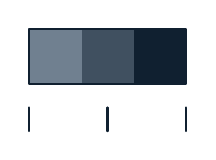
\begin{tikzpicture}[color=iconfg, draw=iconfg, line width=1.3pt, line cap=round, line join=round, >=Stealth, x=1mm,y=1mm]
  \fill[iconfg30] (-10,1) rectangle (-3.3,8);
  \fill[iconfg60] (-3.3,1) rectangle (3.3,8);
  \fill[iconfg] (3.3,1) rectangle (10,8);
  \draw[thick] (-10,1) rectangle (10,8);
  \draw[thick] (-10,-2) -- (-10,-5);
  \draw[thick] (0,-2) -- (0,-5);
  \draw[thick] (10,-2) -- (10,-5);
\end{tikzpicture}
\end{document}
